\section{Problem 1: Perceptual Losses from Pre-trained CNN Features}
\label{sec:p1}

A perceptual loss compares two images in the feature space of a pre-trained network instead of in pixel space~\cite{johnson2016perceptual,zhang2018lpips}.
The hope is that feature distances follow human judgment better than $\ell_1$ or $\ell_2$ distances on pixels.
This section tests that hope for two nuisances a human barely notices, a 1-pixel translation and weak additive noise, and then designs a feature that tolerates atmospheric turbulence.

%-------------------------------------------------------------------------
\subsection{Pixel losses under a 1-pixel translation}
\label{sec:p1-shift}

We used a $4032\times3024$ photograph (\cref{fig:p1-original}), well above the required $1920\times1080$.
Intensities are scaled to $[0,1]$.
The translated image $x'$ is the original $x$ moved 1 pixel to the left, $x'(i,j)=x(i,j+1)$ (\cref{fig:p1-shift}).
\Cref{tab:p1-pixel-loss} lists the $\ell_1$ and $\ell_2$ losses between the two images.

The two images look identical, yet the pixel losses are far from zero.
The MSE of $0.00217$ corresponds to a PSNR of $26.6$\,dB.
That is about the same as adding Gaussian noise with $\sigma=0.05$ (PSNR $26.1$\,dB in \cref{tab:p1-noise}), which is clearly visible (\cref{fig:p1-noise-maps}).
Pixel losses therefore judge an invisible translation as badly as visible noise, because every edge and texture in the image lands on a different pixel.

\begin{figure}[t]
  \centering
  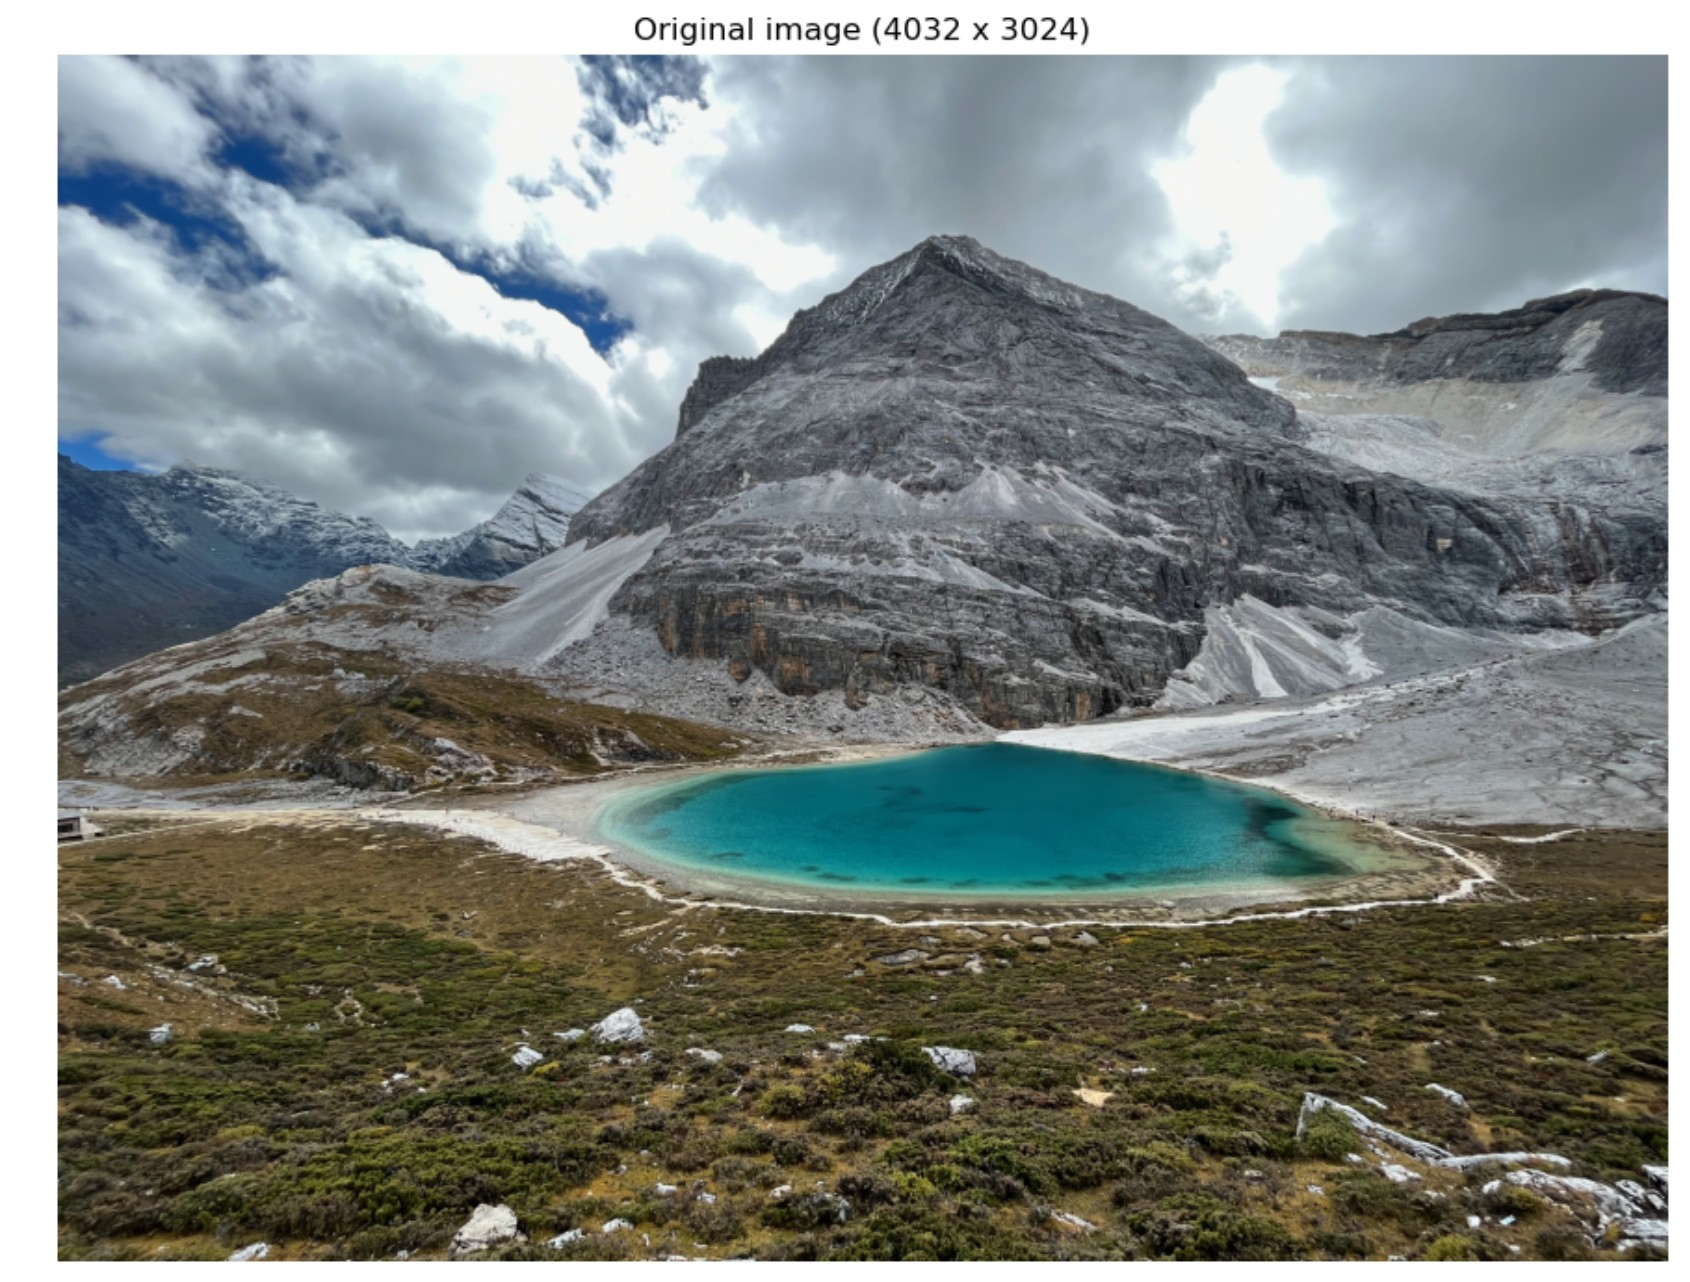
\includegraphics[width=\linewidth]{figs/p1_original.jpg}
  \caption{The test image used throughout Problem 1 ($4032\times3024$ pixels).}
  \label{fig:p1-original}
\end{figure}

\begin{figure}[t]
  \centering
  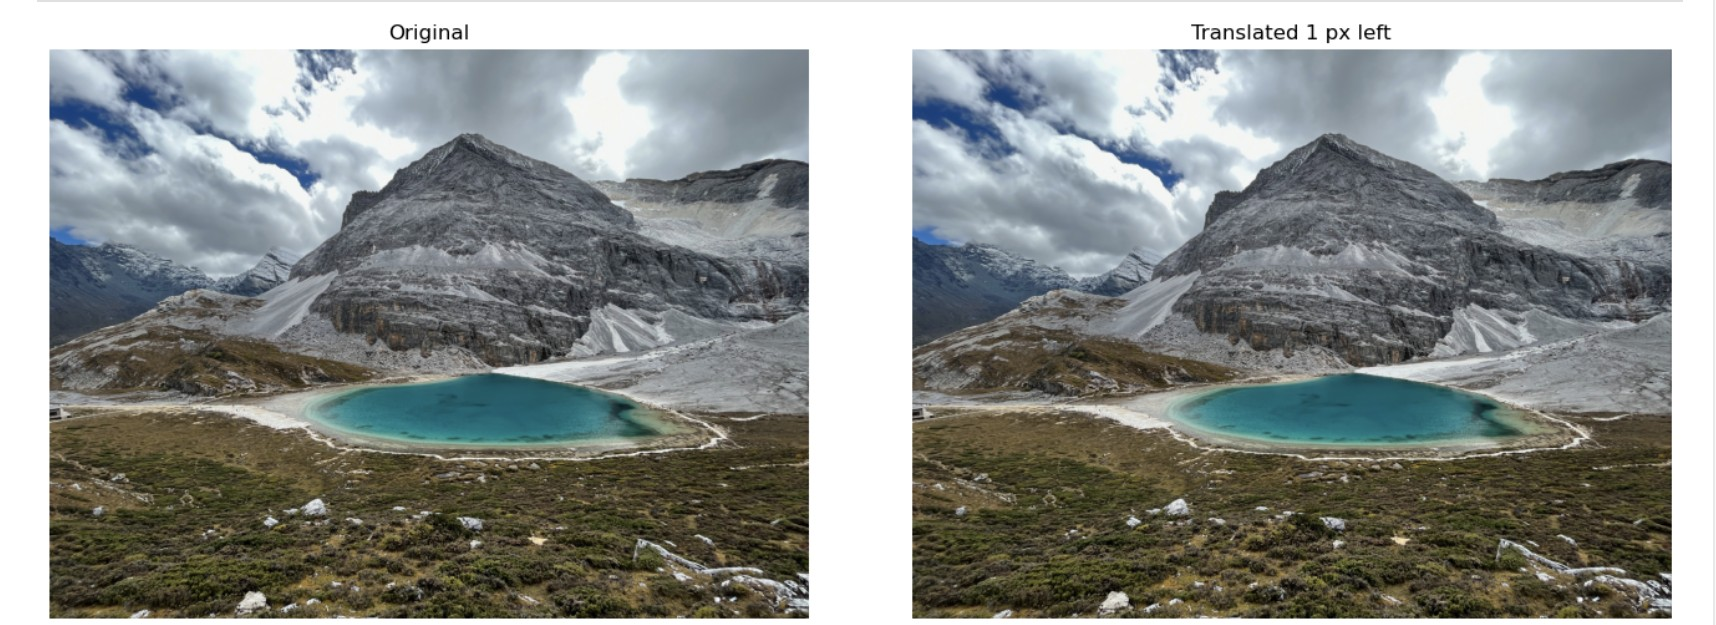
\includegraphics[width=\linewidth]{figs/p1_shift.jpg}
  \caption{Original image (left) and the same image translated 1 pixel to the left (right). The difference is invisible.}
  \label{fig:p1-shift}
\end{figure}

\begin{table}[t]
  \centering
  \small
  \begin{tabular}{@{}lr@{}}
    \toprule
    Loss between $x'$ and $x$ & Value \\
    \midrule
    $\ell_1$, sum $\sum|x'-x|$ & 906{,}791.37 \\
    $\ell_1$, mean (MAE) & 0.024790 \\
    $\ell_2$, sum of squares $\sum(x'-x)^2$ & 79{,}364.72 \\
    $\ell_2$, mean (MSE) & 0.002170 \\
    $\ell_2$ norm $\|x'-x\|_2$ & 281.72 \\
    \bottomrule
  \end{tabular}
  \caption{Pixel losses between the original image and its 1-pixel translation (RGB, intensities in $[0,1]$, $4032\times3024\times3$ values).}
  \label{tab:p1-pixel-loss}
\end{table}

%-------------------------------------------------------------------------
\subsection{Feature-space change in VGG-16}
\label{sec:p1-vgg}

We used the ImageNet-pre-trained VGG-16~\cite{simonyan2015vgg} from torchvision and extracted features after the last ReLU of each of the first four convolution blocks: \relu{1_2}, \relu{2_2}, \relu{3_3} and \relu{4_3} (\cref{fig:p1-vgg}).
These are the layers used by the classic perceptual and LPIPS losses~\cite{johnson2016perceptual,zhang2018lpips}.
They sample the network from edge-like low-level features (full resolution, 64 channels) to part-like mid-level features (1/8 resolution, 512 channels).
Both images were cropped to the $3024\times4031$ region they share, so the comparison contains no border effects, and were normalized with the ImageNet mean and standard deviation.
For each representation $\phi$ we report the mean $\ell_1$ change, the MSE and the scale-free relative change $\|\phi(x')-\phi(x)\|_2/\|\phi(x)\|_2$, which makes pixels and the four feature maps comparable.

\begin{figure*}[t]
  \centering
  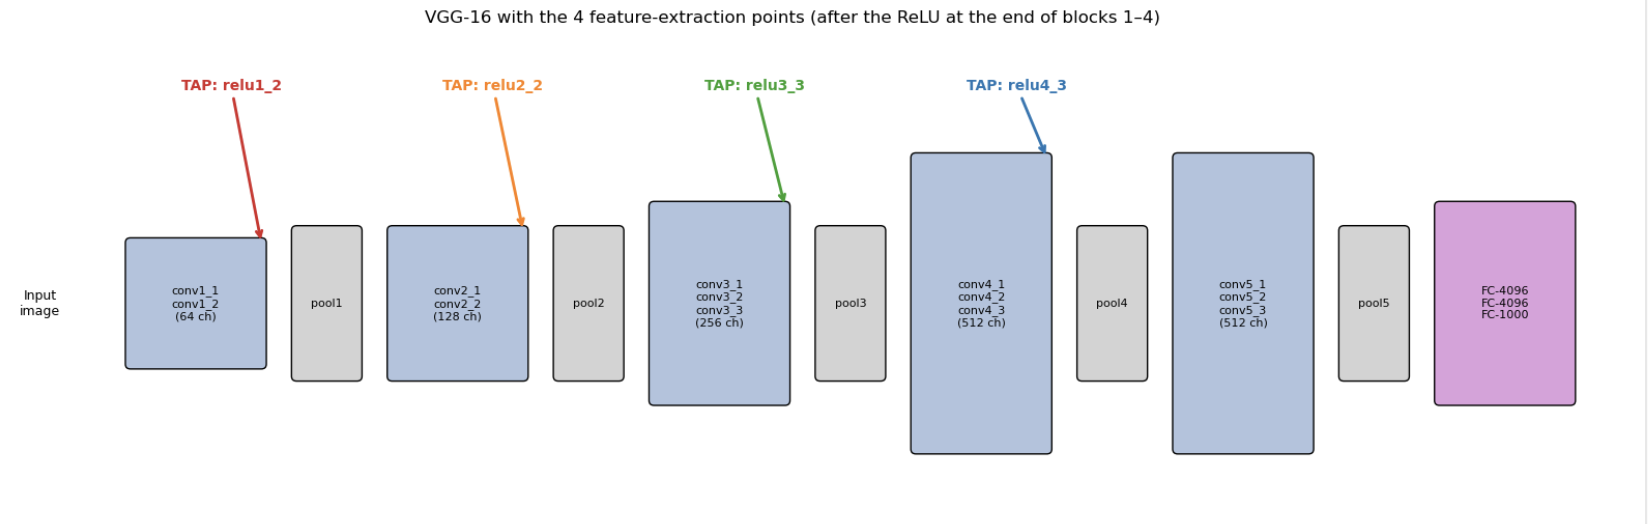
\includegraphics[width=\textwidth]{figs/p1_vgg_taps.png}
  \caption{VGG-16 architecture with the four feature-extraction points used in this report: the ReLU outputs at the end of blocks 1--4. Blue: convolution blocks, gray: max-pooling, purple: fully connected layers.}
  \label{fig:p1-vgg}
\end{figure*}

\begin{table}[t]
  \centering
  \small
  \setlength{\tabcolsep}{4pt}
  \begin{tabular}{@{}llrrr@{}}
    \toprule
    Space & Shape & $\ell_1$ (mean) & MSE & Relative \\
    \midrule
    Pixels & $3\times3024\times4031$ & 0.0247 & 0.0021 & 0.090 \\
    \relu{1_2} & $64\times3024\times4031$ & 0.2543 & 0.4468 & \textbf{0.590} \\
    \relu{2_2} & $128\times1512\times2015$ & 0.3779 & 1.1200 & 0.557 \\
    \relu{3_3} & $256\times756\times1007$ & 0.2291 & 0.6633 & 0.379 \\
    \relu{4_3} & $512\times378\times503$ & 0.0447 & 0.0494 & 0.317 \\
    \bottomrule
  \end{tabular}
  \caption{Change caused by the 1-pixel translation in pixel space and in the four VGG-16 feature spaces. ``Relative'' is $\|\phi(x')-\phi(x)\|_2/\|\phi(x)\|_2$.}
  \label{tab:p1-vgg}
\end{table}

\begin{figure}[t]
  \centering
  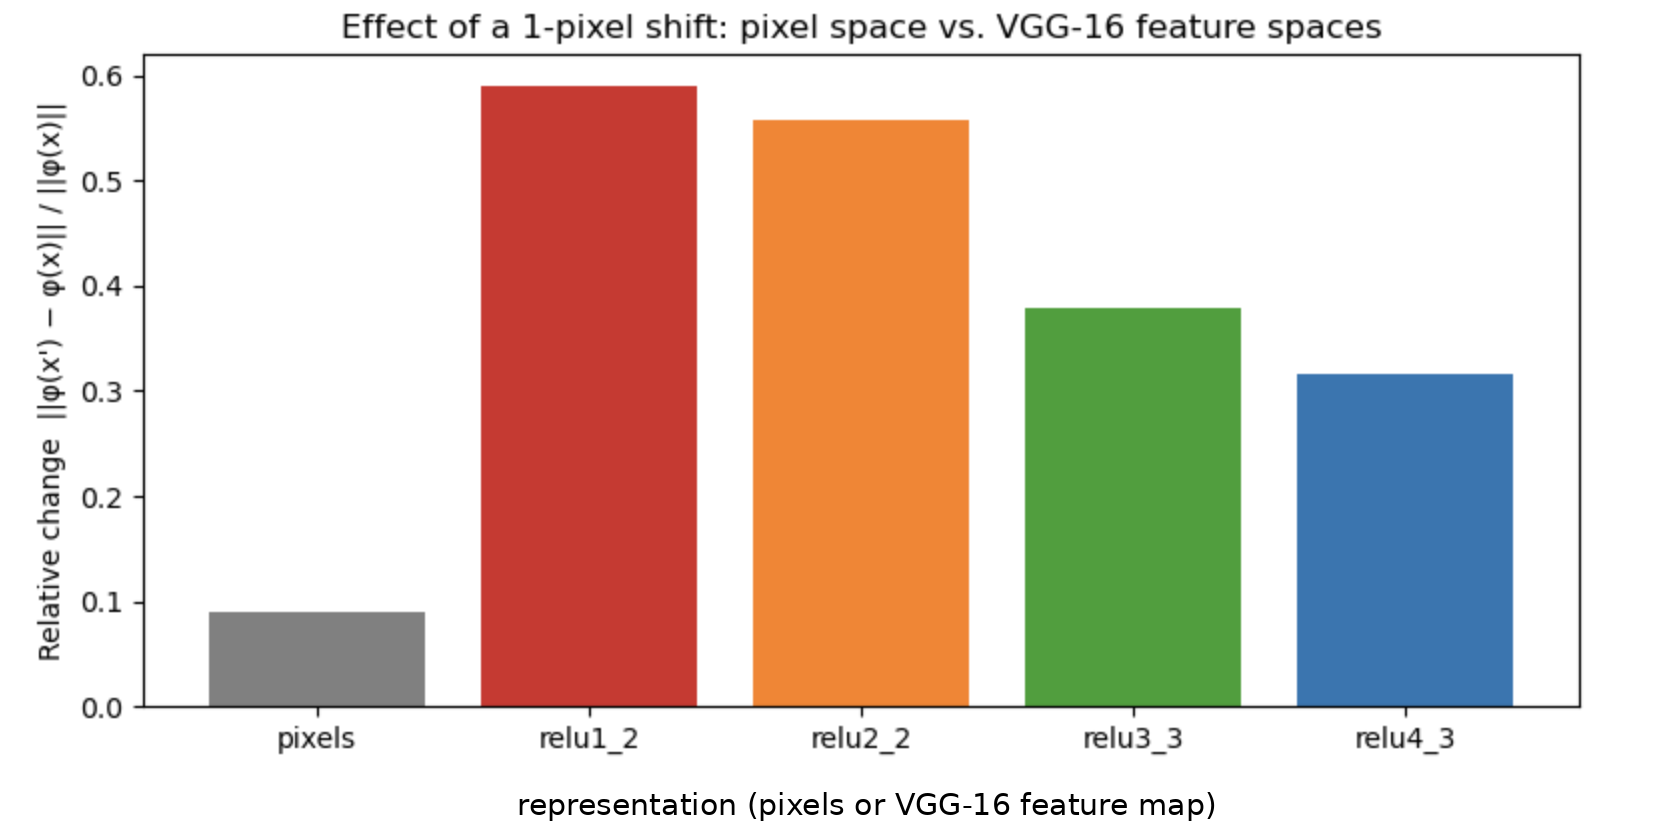
\includegraphics[width=\linewidth]{figs/p1_shift_features.png}
  \caption{Relative change caused by a 1-pixel translation. Every VGG-16 feature map changes 3.5--6.6 times more than the pixels.}
  \label{fig:p1-shift-features}
\end{figure}

\paragraph{Observation.}
\Cref{tab:p1-vgg} and \cref{fig:p1-shift-features} show the opposite of what a perceptual loss should do.
The translation changes the pixels by 9.0\%, but it changes \relu{1_2} by 59\% and \relu{4_3} by 32\%.
VGG features therefore amplify the imperceptible shift instead of ignoring it.
The sensitivity drops with depth, but even the deepest layer is 3.5 times more sensitive than the pixels.

\paragraph{Why it happens.}
We ran four diagnostic checks (\cref{tab:p1-checks}); they were computed in a separate run, so their absolute values differ slightly from \cref{tab:p1-vgg}.
\begin{enumerate}[nosep,leftmargin=*]
  \item \emph{Check 1.} Two identical images give exactly zero change in every layer, so the pipeline itself adds nothing.
  \item \emph{Check 2: the features are shift-equivariant only on their own grid.}
  Layer $k$ has a cumulative stride of 1, 2, 4 or 8 pixels.
  When the image shift is a multiple of that stride, moving the feature map back by shift/stride cells makes the change almost vanish ($\le0.009$).
  The large change for a 1-pixel shift is therefore not a change of content.
  It is aliasing: max-pooling and stride-2 subsampling cannot represent a shift smaller than their stride, so the sampled values change~\cite{zhang2019blurpool}.
  \relu{1_2} has stride 1 and re-aligns perfectly at every shift.
  Its large raw change comes from its content: it is a bank of edge detectors, and an edge map moved by one pixel no longer overlaps itself.
  \item \emph{Check 3.} The same holds in pixel space: keeping only the high frequencies of the image raises its relative change from 0.145 to 0.611, close to \relu{1_2}'s value.
  \item \emph{Checks 4 and 5.} Averaging each channel over the whole image (global average pooling) makes all layers nearly invariant (change $\le3.8\%$), so the sensitivity is purely spatial.
  The deeper layers are sparser (55\% to 92\% exact zeros), yet they change less, because each activation summarizes a larger receptive field and lies on a coarser grid.
\end{enumerate}

\begin{table*}[t]
  \centering
  \small
  \setlength{\tabcolsep}{6pt}
  \begin{tabular}{@{}lcccc@{}}
    \toprule
    \multicolumn{5}{@{}l}{\textbf{Check 2:} relative change, raw / re-aligned by shift/stride cells} \\
    Shift (px) & \relu{1_2} & \relu{2_2} & \relu{3_3} & \relu{4_3} \\
    \midrule
    1  & 0.613 / 0.000 & 0.595 / n/a   & 0.400 / n/a   & 0.342 / n/a \\
    2  & 0.881 / 0.000 & 0.918 / 0.000 & 0.602 / n/a   & 0.400 / n/a \\
    4  & 0.992 / 0.000 & 1.146 / 0.000 & 0.915 / 0.002 & 0.488 / n/a \\
    8  & 1.021 / 0.000 & 1.188 / 0.000 & 1.172 / 0.002 & 0.707 / 0.009 \\
    16 & 1.044 / 0.000 & 1.212 / 0.000 & 1.240 / 0.002 & 1.004 / 0.009 \\
    \midrule
    \multicolumn{5}{@{}l}{\textbf{Check 1:} identical images give 0 in all four layers.} \\
    \multicolumn{5}{@{}l}{\textbf{Check 3:} pixel relative change for a 1-px shift: raw 0.145, mean-subtracted 0.309, high-pass (edges only) 0.611.} \\
    \midrule
    & \relu{1_2} & \relu{2_2} & \relu{3_3} & \relu{4_3} \\
    \textbf{Check 4:} global-average-pooled change & 0.00045 & 0.0224 & 0.0245 & 0.0380 \\
    \textbf{Check 5:} fraction of zero activations & 55.3\% & 70.4\% & 84.7\% & 92.0\% \\
    \bottomrule
  \end{tabular}
  \caption{Diagnostic checks for the shift sensitivity of VGG-16. ``n/a'': the shift is not a multiple of the layer's stride, so the map cannot be re-aligned.}
  \label{tab:p1-checks}
\end{table*}

\paragraph{Feature for a perceptual loss.}
We would use \relu{3_3}, ideally compared after a small spatial blur or pooling of the feature maps.
Of the four layers it gives the best trade-off in our measurements.
It is far less sensitive to the imperceptible shift than \relu{1_2} and \relu{2_2} (0.38 vs.\ 0.59 and 0.56).
Its response to noise grows much more slowly than that of the shallow layers (\cref{sec:p1-noise}).
Unlike \relu{4_3}, it keeps a 1/4-resolution map, so it can still localize small errors, which matters for restoration tasks.
The checks also show how to make it better: the remaining sensitivity is caused by aliasing, so anti-aliased downsampling~\cite{zhang2019blurpool} or spatial pooling should remove most of it.
We use exactly this observation in \cref{sec:p1-turb}.

%-------------------------------------------------------------------------
\subsection{Robustness to additive noise}
\label{sec:p1-noise}

We added zero-mean Gaussian noise with standard deviation $\sigma\in\{0.01,0.02,0.05,0.1,0.2,0.3\}$ to the image and measured the change of each representation (\cref{tab:p1-noise,fig:p1-noise-curves,fig:p1-noise-maps}).

\begin{table}[t]
  \centering
  \small
  \setlength{\tabcolsep}{3.5pt}
  \resizebox{\linewidth}{!}{%
  \begin{tabular}{@{}ccccccc@{}}
    \toprule
    & & \multicolumn{5}{c}{Relative change $\|\Delta\phi\|_2/\|\phi\|_2$} \\
    \cmidrule(l){3-7}
    $\sigma$ & PSNR (dB) & Pixels & \relu{1_2} & \relu{2_2} & \relu{3_3} & \relu{4_3} \\
    \midrule
    0.01 & 40.0 & 0.020 & 0.114 & 0.217 & 0.251 & 0.296 \\
    0.02 & 34.0 & 0.039 & 0.223 & 0.378 & 0.404 & 0.458 \\
    0.05 & 26.1 & 0.097 & 0.499 & 0.746 & 0.688 & 0.733 \\
    0.10 & 20.3 & 0.190 & 0.874 & 1.197 & 0.924 & 0.929 \\
    0.20 & 14.7 & 0.360 & 1.485 & 1.887 & 1.180 & 1.083 \\
    0.30 & 11.9 & 0.499 & 1.958 & 2.421 & 1.370 & 1.161 \\
    \midrule
    \multicolumn{2}{@{}l}{MSE growth, $\sigma{:}\ 0.01\!\to\!0.3$} & $646\times$ & $297\times$ & $124\times$ & $30\times$ & $15\times$ \\
    \bottomrule
  \end{tabular}}
  \caption{Change of each representation under additive Gaussian noise. The last row is the ratio of the MSE at $\sigma=0.3$ to the MSE at $\sigma=0.01$.}
  \label{tab:p1-noise}
\end{table}

\begin{figure*}[t]
  \centering
  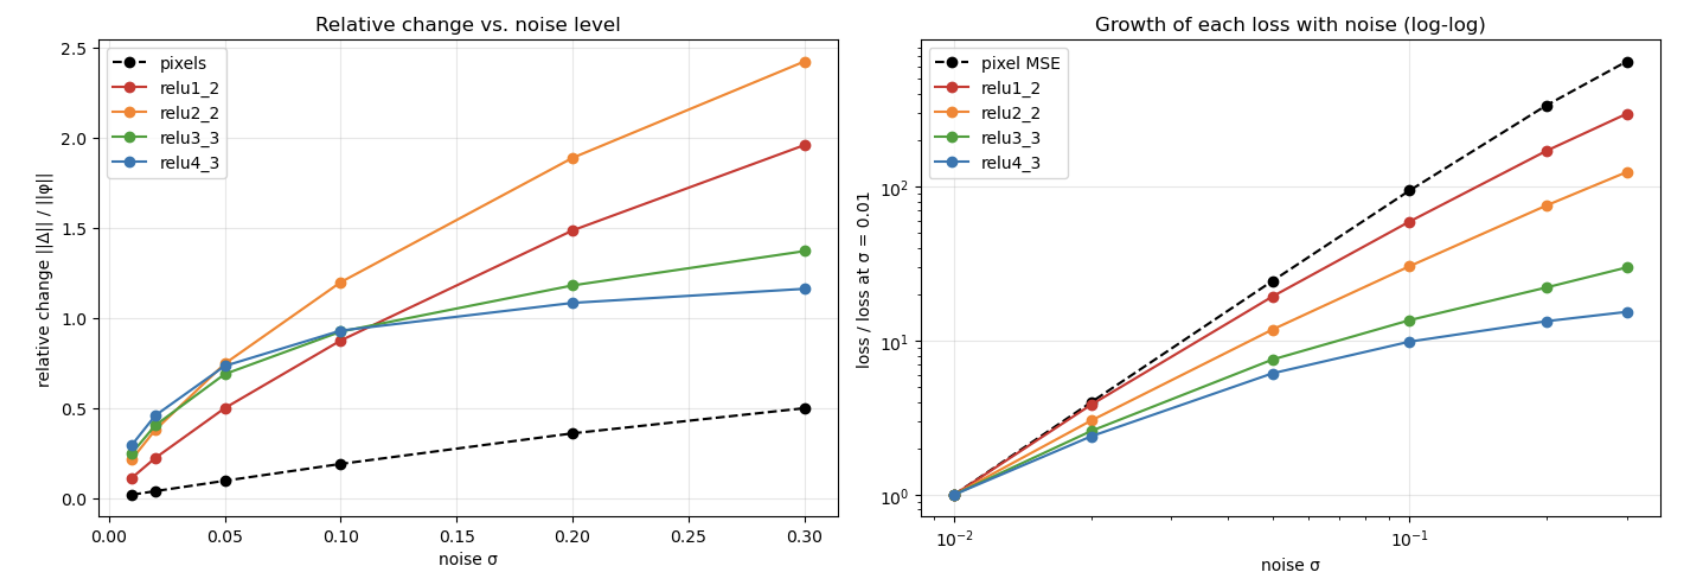
\includegraphics[width=0.92\textwidth]{figs/p1_noise_curves.png}
  \caption{Left: relative change of each representation versus noise level. Right: each loss normalized by its value at $\sigma=0.01$ (log-log axes). Pixel MSE grows as $\sigma^2$; the deep features grow far more slowly and saturate.}
  \label{fig:p1-noise-curves}
\end{figure*}

\begin{figure*}[t]
  \centering
  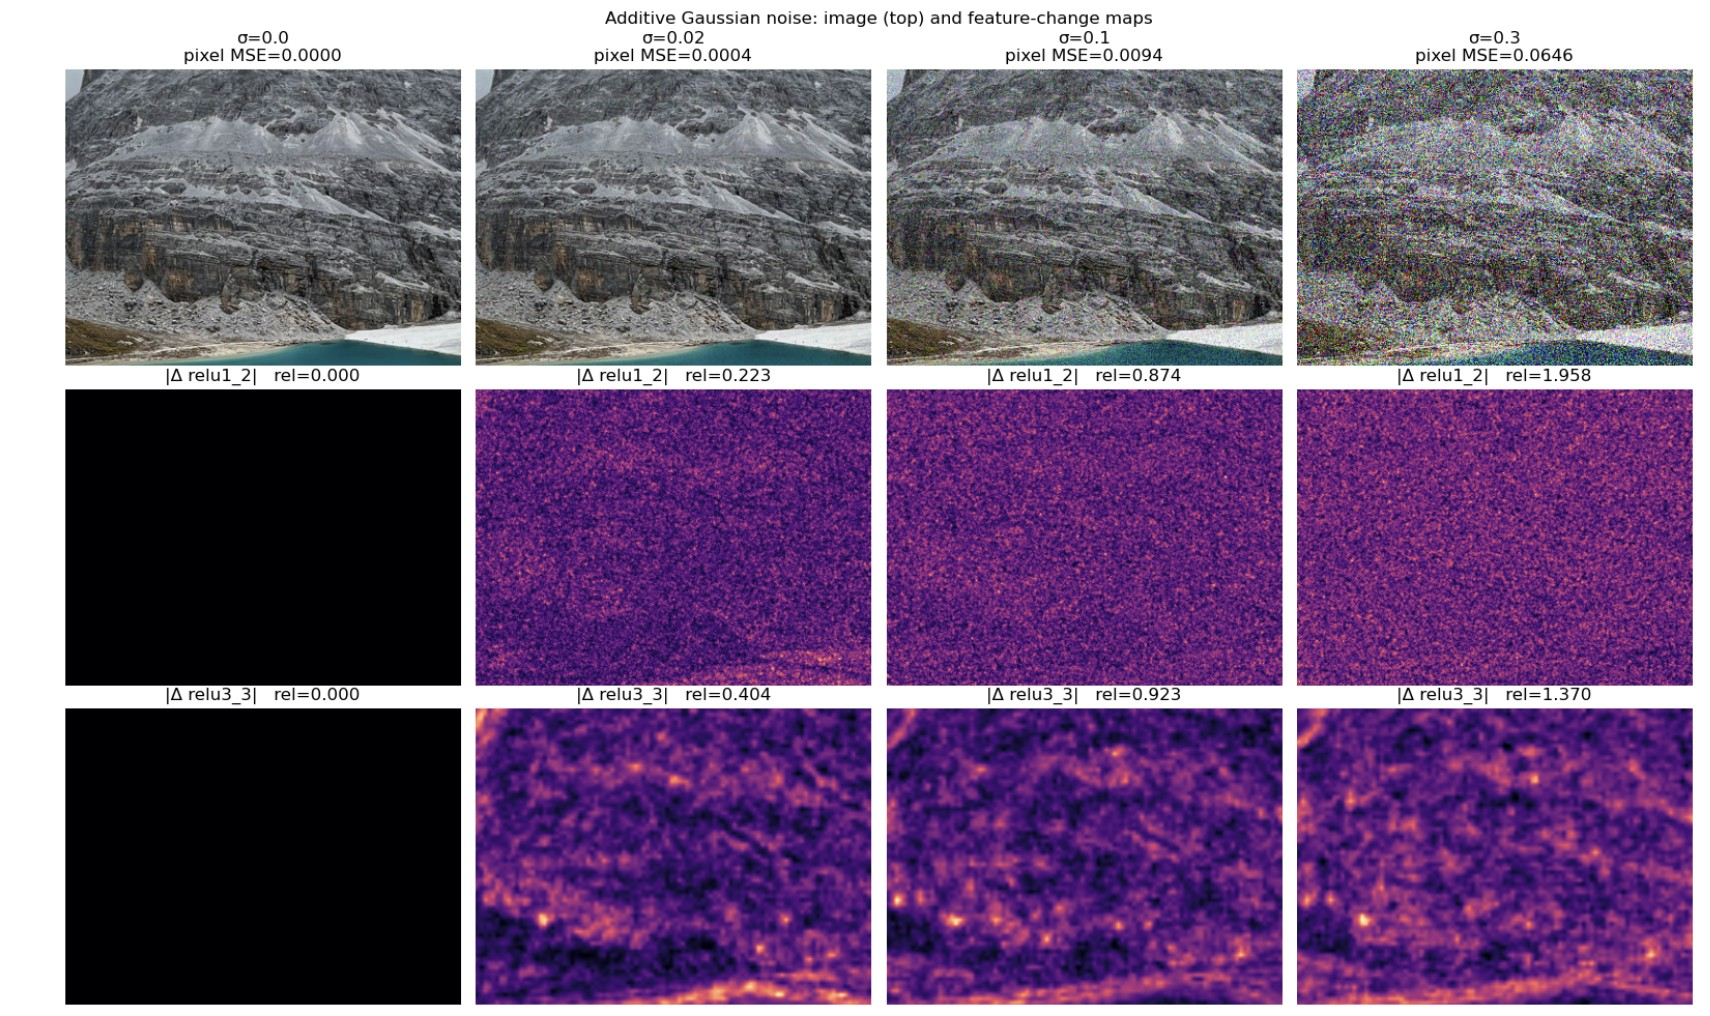
\includegraphics[width=0.85\textwidth]{figs/p1_noise_maps.jpg}
  \caption{Qualitative noise test on a crop of the image. Top: noisy images for $\sigma=0$, 0.02, 0.1 and 0.3. Middle and bottom: where the \relu{1_2} and \relu{3_3} features change (brighter = larger change). \relu{1_2} changes uniformly everywhere, like the noise itself; the \relu{3_3} change follows the image structure (rock texture, shoreline) and keeps the same pattern as $\sigma$ grows.}
  \label{fig:p1-noise-maps}
\end{figure*}

\paragraph{Quantitative results.}
Three effects stand out.
\begin{enumerate}[nosep,leftmargin=*]
  \item \emph{Over-reaction to invisible noise.} At $\sigma=0.01$ (PSNR 40\,dB, invisible), the features already change by 11--30\%, while the pixels change by 2\%. This is the same magnitude as the 1-pixel shift: VGG features react strongly to any small high-frequency perturbation.
  \item \emph{Saturation with depth.} When $\sigma$ grows 30 times, the pixel MSE grows $646\times$, close to the $\sigma^2$ law (clipping to $[0,1]$ keeps it below $900\times$). The MSE of \relu{1_2} grows $297\times$, \relu{2_2} $124\times$, \relu{3_3} $30\times$ and \relu{4_3} only $15\times$ (\cref{fig:p1-noise-curves}, right). The relative change of \relu{4_3} goes from 0.93 to only 1.16 between $\sigma=0.1$ and $0.3$, although the image gets visibly much worse.
  \item \emph{Most and least sensitive layers.} \relu{2_2} is the most sensitive layer at every $\sigma\ge0.05$; \relu{4_3} is the least sensitive for $\sigma\ge0.2$.
\end{enumerate}

\paragraph{Qualitative results.}
\Cref{fig:p1-noise-maps} shows where the features change.
The \relu{1_2} change is spatially uniform speckle: the layer encodes the noise itself.
The \relu{3_3} change is concentrated on textured regions and edges and keeps the same spatial pattern as $\sigma$ grows.
The deeper layer thus reports where the image \emph{structure} is corrupted, which is closer to what a human notices.

\paragraph{Conclusion.}
None of the four layers is robust to noise in the sense of ignoring invisible perturbations; all over-react at $\sigma=0.01$.
The deeper layers have the more useful behavior: they flag noise once, concentrate the change on structure, and do not keep growing quadratically.
This supports \relu{3_3}, possibly combined with \relu{4_3}, as the perceptual feature, with the caveat that deep features cannot rank strong noise levels well because they saturate.

%-------------------------------------------------------------------------
\subsection{A perceptual feature robust to atmospheric turbulence}
\label{sec:p1-turb}

\paragraph{What turbulence does.}
DAATSim~\cite{saha2025daatsim} models turbulence as two effects.
\emph{Tilt} is a smooth random warp: every region moves by a different sub-pixel to few-pixel amount.
\emph{Blur} is a spatially varying blur from Zernike-based point-spread functions.
The scene content does not change.
Tilt is made of exactly the small, non-stride-aligned local shifts that \cref{sec:p1-vgg} showed VGG-16 features to be most sensitive to.
We therefore expect standard VGG features to judge a turbulent copy as a large change.

\paragraph{Dataset.}
We took the 100 photographs of the DIV2K validation set~\cite{agustsson2017div2k} and cut 8 random square crops from each, resized to $256\times256$, for 800 clean images (\cref{fig:p1-turb-data}).
The split is by source photograph, so no photo appears in both sets: 80 photos (640 crops) for training and 20 photos (160 crops) for testing.
Each training crop has 3 turbulent versions with $r_0$ drawn log-uniformly from $[0.02,0.1]$.
Each test crop has one version at each of five fixed strengths $r_0\in\{0.1,0.05,0.03,0.02,0.01\}$.
With DAATSim's aperture $D=0.2$, these correspond to $D/r_0\in\{2,4,6.7,10,20\}$.
The strongest level, $D/r_0=20$, is outside the training range and tests generalization.

\begin{figure*}[t]
  \centering
  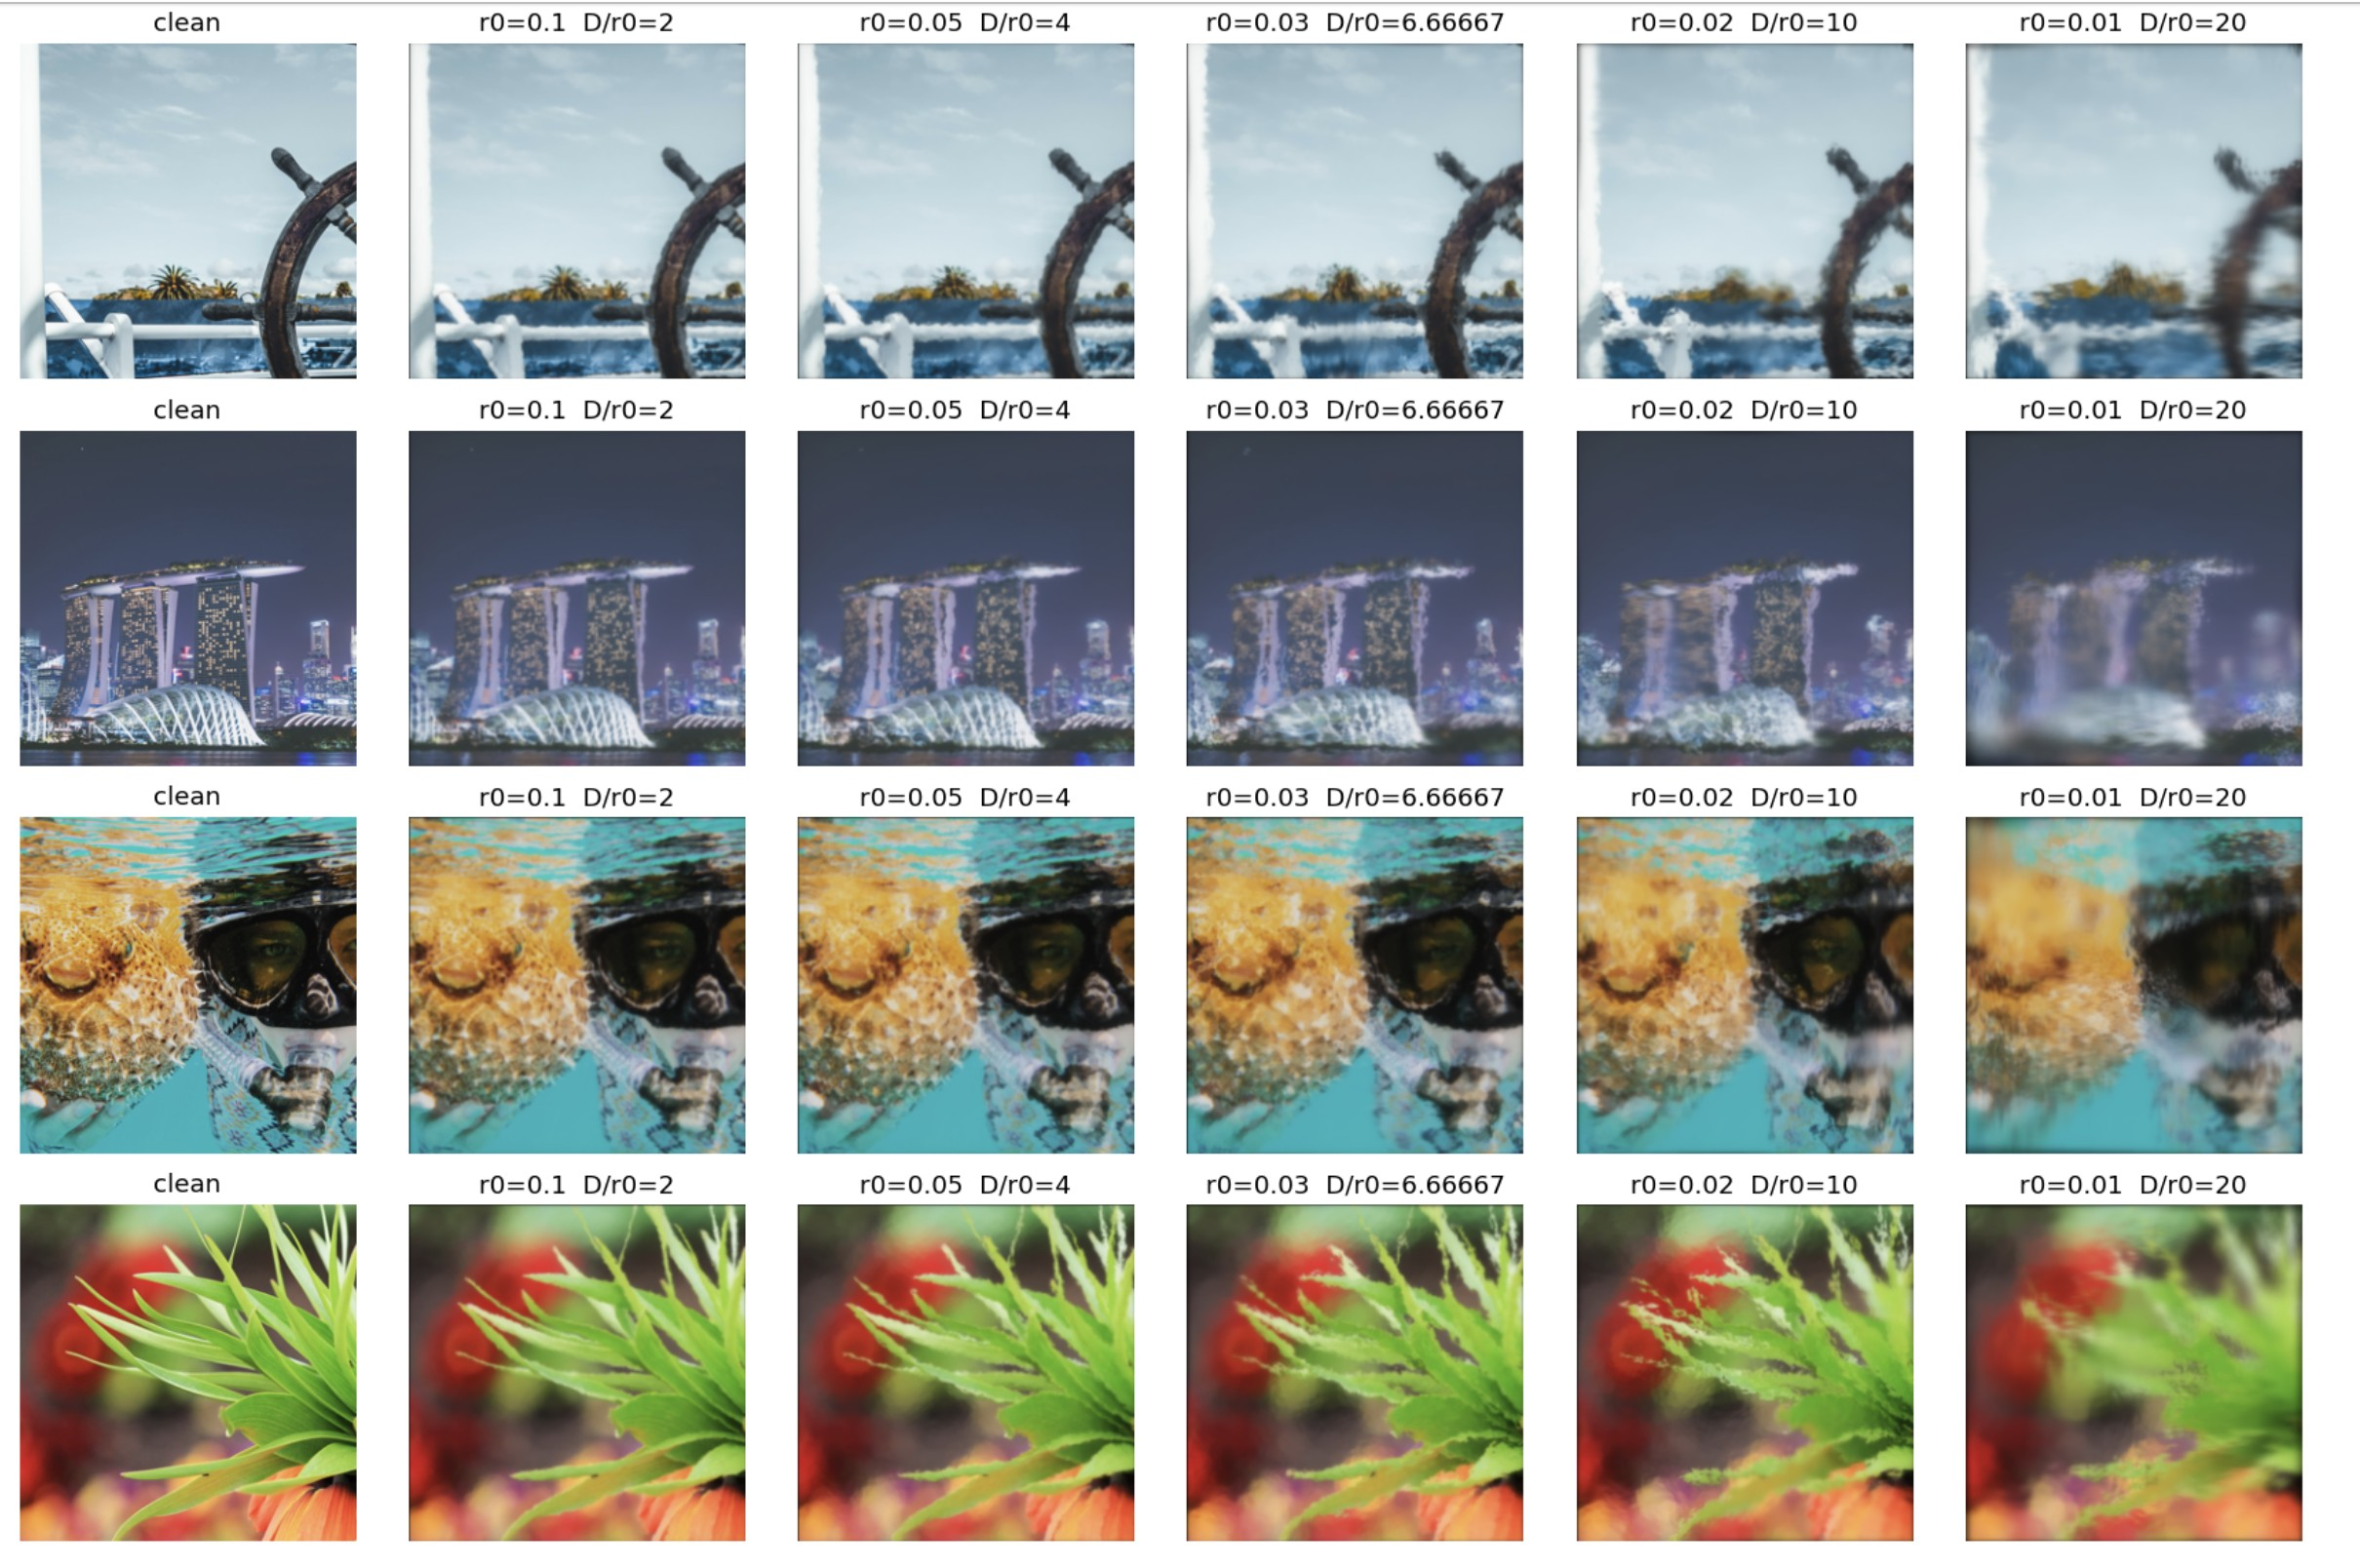
\includegraphics[width=0.8\textwidth]{figs/p1_turb_dataset.jpg}
  \caption{Examples from our turbulence dataset: clean $256\times256$ crops (left column) and DAATSim renderings at the five test strengths (smaller $r_0$, larger $D/r_0$ = stronger turbulence). Tilt bends straight structures (railings, building edges); blur removes fine texture.}
  \label{fig:p1-turb-data}
\end{figure*}

\paragraph{Proposed feature.}
The feature has three parts.
\begin{enumerate}[nosep,leftmargin=*]
  \item \emph{Anti-aliased trunk.} A frozen ImageNet VGG-16 in which every $2\times2$ max-pooling is replaced by max $\rightarrow$ blur $\rightarrow$ subsample (MaxBlurPool~\cite{zhang2019blurpool}). This directly targets the aliasing measured in \cref{tab:p1-checks}.
  \item \emph{Multi-scale head.} \relu{2_2} (downsampled with an anti-aliased blur-pool) and \relu{3_3} are concatenated. Two $3\times3$ convolutions turn them into a 128-dimensional, unit-normalized feature map at 1/4 resolution. The head has 1.18\,M trainable parameters. Its $3\times3$ receptive field lets it learn to tolerate the local displacements caused by tilt.
  \item \emph{Dense contrastive training} (InfoNCE~\cite{oord2018cpc,wang2021densecl}, \cref{lst:p1-infonce}). At 64 random locations $p$ per image, the feature of the clean image at $p$ must match the feature of the turbulent image at the same $p$, and so must two different turbulence realizations. It must \emph{not} match any other sampled location, in the same image or in the other images of the batch.
\end{enumerate}
The positive pairs teach invariance to turbulence.
The negatives force every location to keep identifying its own content, so the feature cannot collapse to a constant and still responds to real changes.
Turbulence is a nuisance transformation and the simulator provides unlimited (clean, turbulent) pairs, so the network can be told exactly which changes to ignore.

\paragraph{Training.}
Only the head is trained: AdamW~\cite{loshchilov2019adamw}, learning rate $10^{-3}$, weight decay $10^{-4}$, cosine schedule, 30 epochs, batch of 16 triplets (clean image and two turbulent versions), temperature $\tau=0.1$.
We also trained two ablations: the same head on the original VGG pooling (\emph{w/o anti-alias}), and the head trained without negatives (\emph{invariance-only}, which only pulls the two views together).

\begin{lstlisting}[caption={Dense InfoNCE loss (from \texttt{p4lib.py}, shortened; \texttt{gather} picks the sampled locations).},label={lst:p1-infonce},float=t]
def dense_infonce(za, zb, n_loc=64, tau=0.1):
    # za, zb: (B, D, h, w) unit-norm feature maps
    # of two views (clean / turbulent) of a batch
    ...  # idx: n_loc random locations per image
    qa = gather(za, idx)    # (B * n_loc, D)
    qb = gather(zb, idx)    # same places, view b
    logits = qa @ qb.t() / tau  # all pairs
    # positive = same location of the same image
    target = torch.arange(len(qa))
    loss_ab = F.cross_entropy(logits, target)
    loss_ba = F.cross_entropy(logits.t(), target)
    return 0.5 * (loss_ab + loss_ba)
\end{lstlisting}

\paragraph{How robustness is measured.}
A feature that outputs a constant is perfectly invariant and useless, so invariance alone is not a good measure.
For every held-out test image $x$ we compute three distances:
$d(x,T(x))$ to its turbulent version, which should be small;
$d(x,\mathrm{edit}(x))$ to a copy whose $64\times64$ patch is replaced by content from another scene, a real visible change, which should be large;
and $d(x,y)$ to a completely different image, which sets the scale.
We report $\mathrm{AUC}_\mathrm{edit}=P\big(d(x,T(x))<d(x,\mathrm{edit}(x))\big)$, where 1 means turbulence is always judged a smaller change than a real edit, and the ratio $\mathrm{median}\,d(x,T(x))/\mathrm{median}\,d(x,y)$, where lower means more invariant.
We compare against the standard features from the previous parts: pixel MSE, blurred pixels (Gaussian, $\sigma=2$), each VGG layer, an LPIPS-style average over the four layers, and the anti-aliased VGG \relu{3_3} without training.

\begin{figure*}[t]
  \centering
  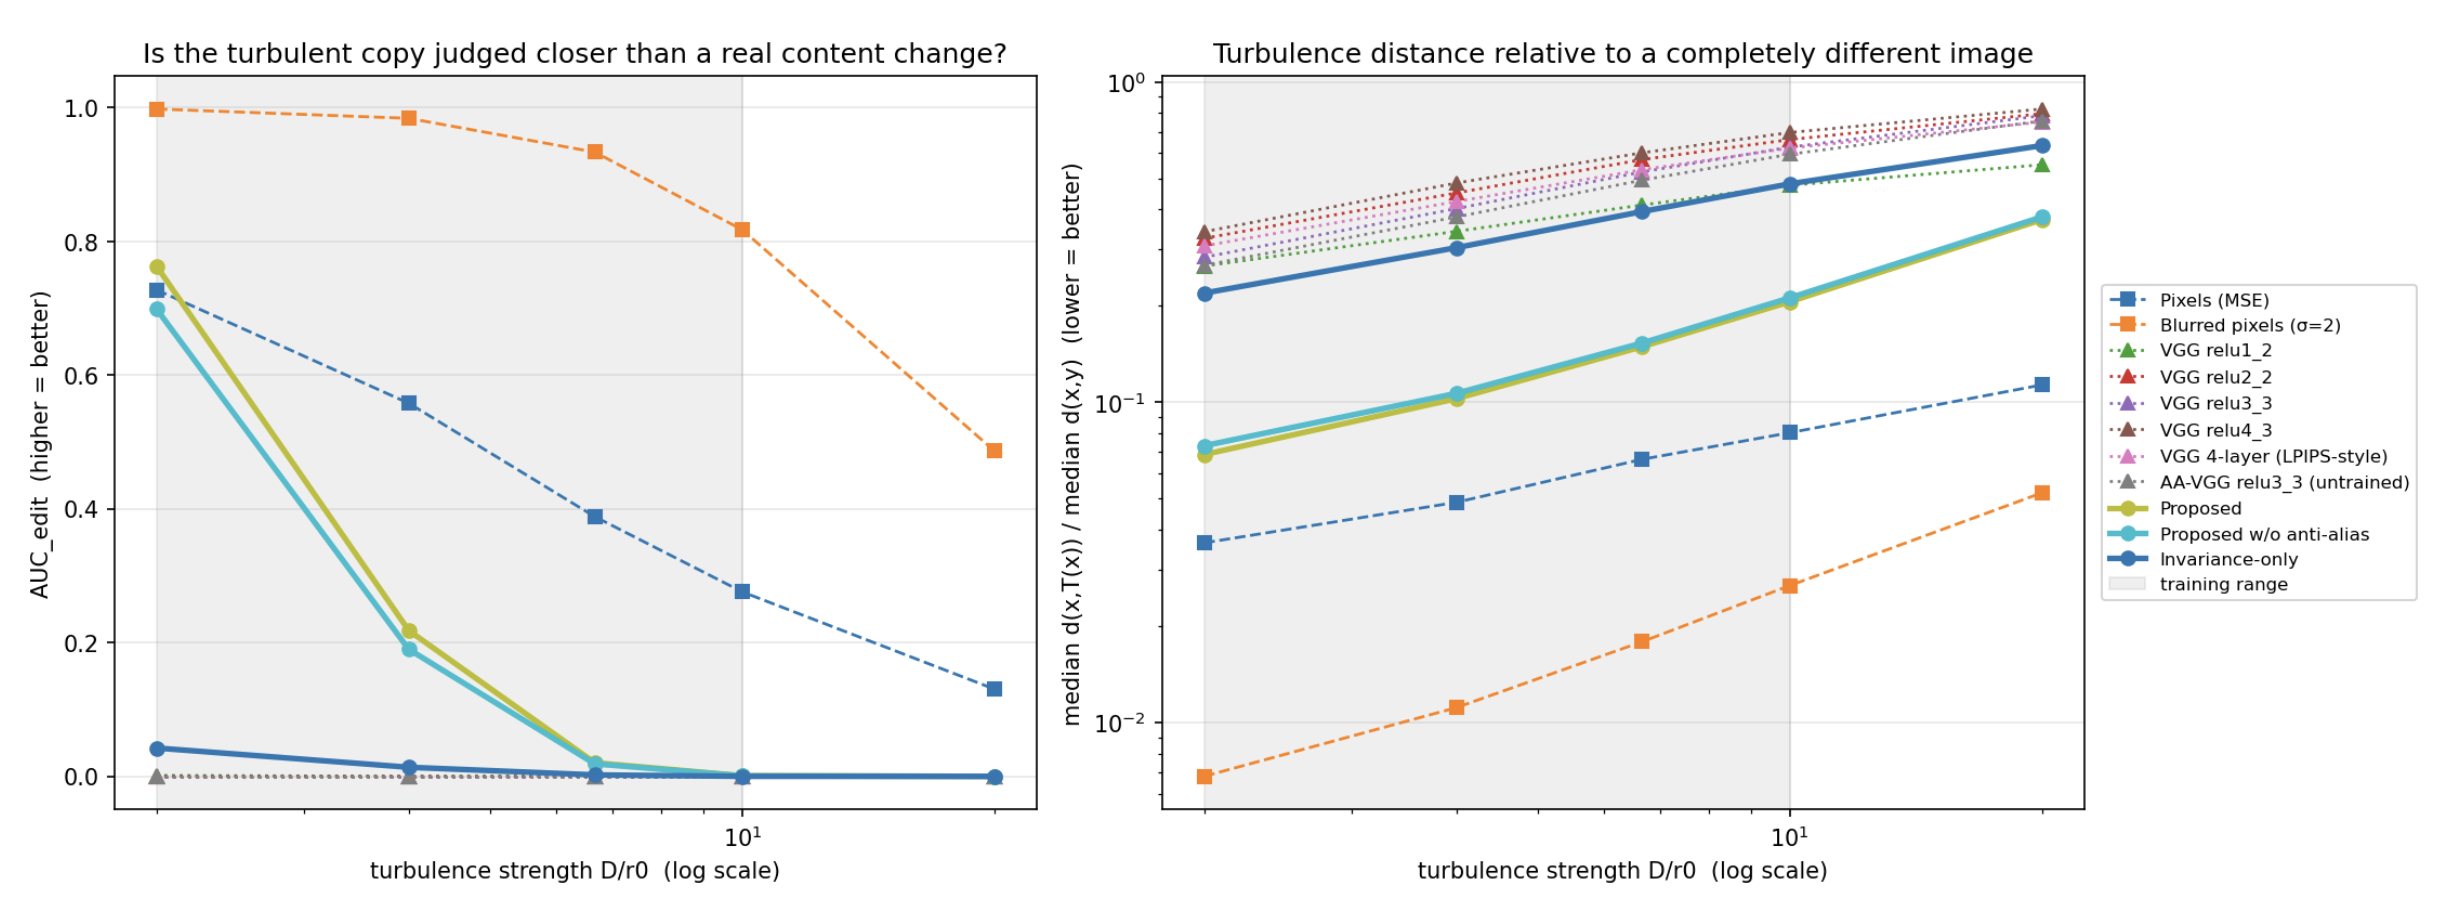
\includegraphics[width=\textwidth]{figs/p1_turb_quant.png}
  \caption{Turbulence robustness on the 160 held-out test images, per turbulence strength. Left: $\mathrm{AUC}_\mathrm{edit}$, the probability that the turbulent copy is judged closer than a $64\times64$ content edit (higher is better). Right: distance to the turbulent copy divided by the distance to a different image (lower is better). The gray band is the training range of $D/r_0$.}
  \label{fig:p1-turb-quant}
\end{figure*}

\begin{figure*}[t]
  \centering
  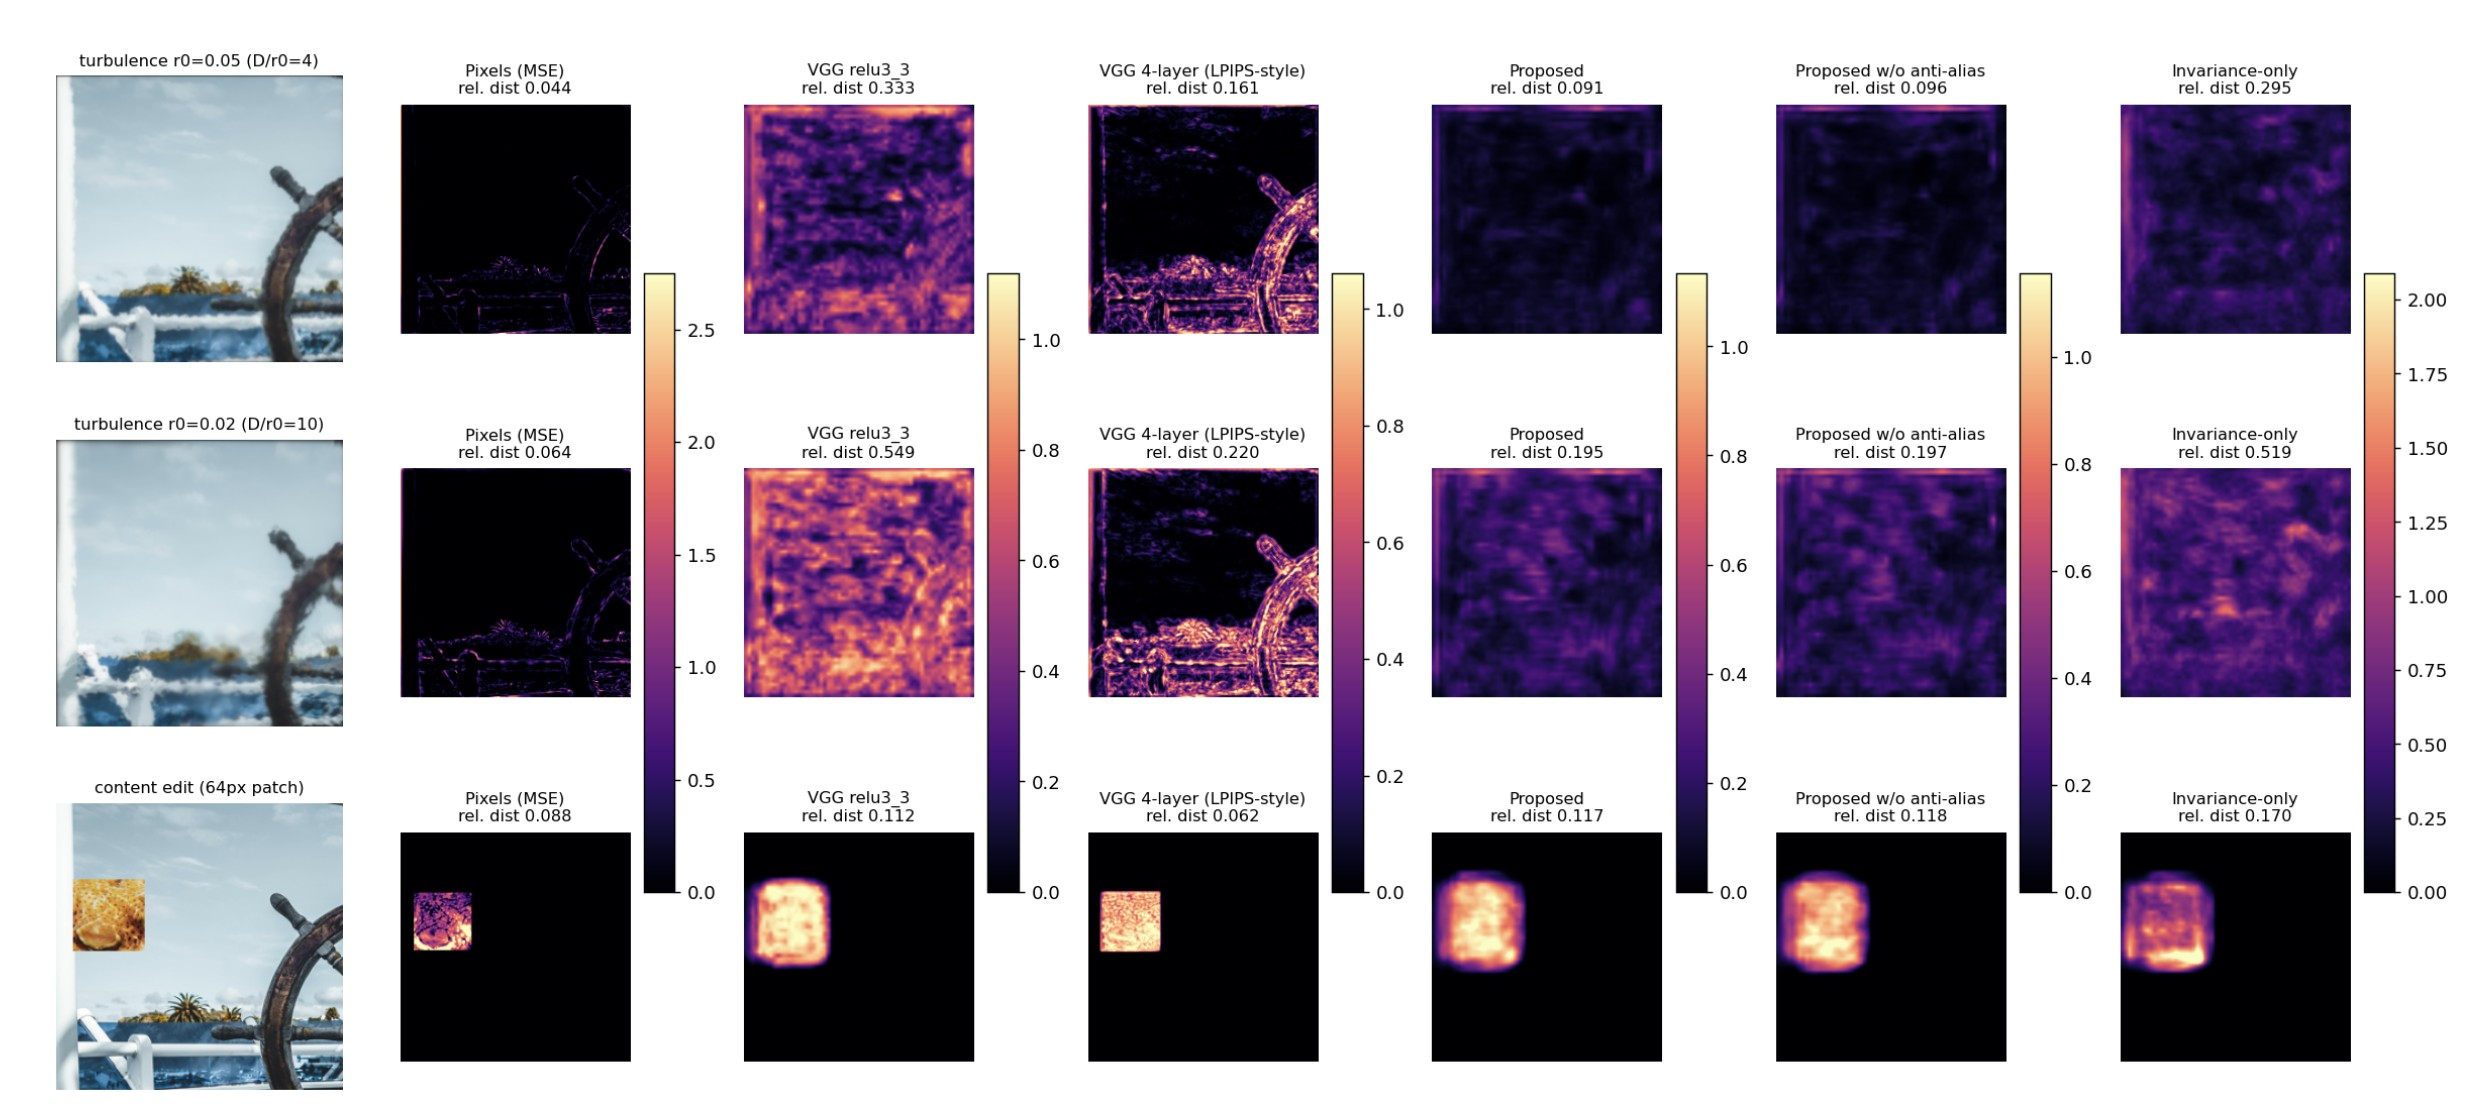
\includegraphics[width=\textwidth]{figs/p1_turb_qual.jpg}
  \caption{Where each feature changes, for two turbulence strengths (rows 1--2) and a content edit (row 3) of the same test image. Each map is divided by that feature's distance to a different image, and each column shares one color scale. Ideal: dark for turbulence, bright only on the edited patch. The number above each map is the relative distance (also listed in \cref{tab:p1-turb-example}).}
  \label{fig:p1-turb-qual}
\end{figure*}

\begin{table}[t]
  \centering
  \small
  \setlength{\tabcolsep}{4pt}
  \begin{tabular}{@{}lccc@{}}
    \toprule
    Feature & \makecell{Turb.\\$D/r_0=4$} & \makecell{Turb.\\$D/r_0=10$} & \makecell{Content\\edit} \\
    \midrule
    Pixels (MSE) & 0.044 & 0.064 & 0.088 \\
    VGG \relu{3_3} & 0.333 & 0.549 & 0.112 \\
    VGG 4-layer (LPIPS-style) & 0.161 & 0.220 & 0.062 \\
    \textbf{Proposed} & \textbf{0.091} & \textbf{0.195} & 0.117 \\
    Proposed w/o anti-alias & 0.096 & 0.197 & 0.118 \\
    Invariance-only (ablation) & 0.295 & 0.519 & 0.170 \\
    \bottomrule
  \end{tabular}
  \caption{Relative distances for the example of \cref{fig:p1-turb-qual}. A good feature has a turbulence distance below its content-edit distance.}
  \label{tab:p1-turb-example}
\end{table}

\paragraph{Results.}
\Cref{fig:p1-turb-quant} and \cref{fig:p1-turb-qual} summarize the comparison.
\begin{itemize}[nosep,leftmargin=*]
  \item \emph{Standard VGG features fail completely}, as predicted from \cref{sec:p1-vgg}.
  Every VGG layer and the LPIPS-style combination has $\mathrm{AUC}_\mathrm{edit}\approx0$ at every strength.
  Even the mildest turbulence ($D/r_0=2$) is almost always judged a larger change than replacing a $64\times64$ patch with another scene.
  In the example, \relu{3_3} rates turbulence at $D/r_0=4$ three times farther than the edit (0.333 vs.\ 0.112), and its change map lights up the whole image.
  \item \emph{The proposed feature is much more turbulence-invariant than VGG.}
  Its turbulence-to-different-image ratio is about 0.07 at $D/r_0=2$, four times lower than any VGG baseline (0.27--0.33), and stays below them up to $D/r_0=20$, outside the training range.
  It raises $\mathrm{AUC}_\mathrm{edit}$ at $D/r_0=2$ from $\approx0$ to about 0.76.
  In the example, both proposed variants rank mild turbulence below the edit (0.091 vs.\ 0.117), whereas every VGG feature ranks it far above, and the edit response stays localized on the patch.
  \item \emph{Anti-aliasing helps slightly.} Without MaxBlurPool, $\mathrm{AUC}_\mathrm{edit}$ at $D/r_0=2$ drops from about 0.76 to 0.70; the other strengths are almost unchanged.
  \item \emph{The negatives are essential.} The invariance-only ablation reaches $\mathrm{AUC}_\mathrm{edit}\le0.04$ at every strength, and its ratio (0.22 at $D/r_0=2$) is only slightly below the VGG baselines. Without negatives, the head loses the ability to tell content changes from turbulence.
  \item \emph{Limitations: pixel-based distances are hard to beat.} $\mathrm{AUC}_\mathrm{edit}$ of the proposed feature falls to about 0.2 at $D/r_0=4$ and to $\approx0$ from $D/r_0\approx6.7$. Plain pixel MSE is about as good at $D/r_0=2$ (0.73) and better at stronger turbulence (0.56, 0.39, 0.28, 0.13). The simple hand-made baseline of blurred pixels is the best method on $\mathrm{AUC}_\mathrm{edit}$ at all strengths (from $\approx1.0$ at $D/r_0=2$ to 0.49 at $D/r_0=20$) and has the lowest ratio, because low-pass filtering removes most of the tilt and blur difference at once. Our feature fixes the failure of VGG features at mild turbulence, but it does not surpass the pixel-based distances.
\end{itemize}

\paragraph{Discussion.}
The experiments give a clear picture of why the problem is hard.
At strong turbulence, tilt moves content by more pixels than the head's $3\times3$ receptive field at 1/4 resolution can absorb, and blur removes texture that the VGG trunk relies on.
A larger receptive field (more head layers or a feature pyramid), training on stronger turbulence, or combining the learned feature with a low-pass pixel term are natural next steps.
Two caveats apply.
A turbulence-invariant feature is, by design, less sensitive to blur and small misalignments in general, which is a real trade-off for restoration, where blur \emph{should} be penalized.
And training and testing both use DAATSim in uniform (depth-free) mode; real turbulence is depth-dependent and correlated in time, so a sim-to-real gap is likely.
